\documentclass[../main.tex]{subfiles}
\chapter{Herleitung}
\label{c:herleitung}

\section{Homogene Transformationsmatrix}

\begin{figure}
	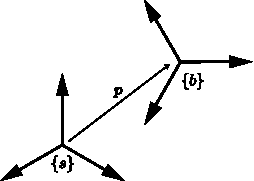
\includegraphics{frames}
	\caption{Transformation von space-frame $\{s\}$ nach body-frame $\{b\}$}
	\label{fig:frames}
\end{figure}

Die in Abbildung \ref{fig:frames} dargestellte Anordnung eines körperfesten Koordinatensystems $\{b\}$ (body-frame) in einem raumfesten Koordinatensystem $\{s\}$ (space-frame) kann beschrieben werden durch die Position $\mathbf{p}$ des body-frames in $\{s\}$-Koordinaten und einer Rotationsmatrix $\mathbf{R}$, welche die Ausrichtung von $\{b\}$ in $\{s\}$-Koordinaten beschreibt (siehe Abb. \ref{fig:frames}).
Die homogene Transformationsmatrix $\mathbf{T}$ ist die kombinierte Repräsentation von Orientierung und Position als Matrix \cite[Ch. 3.3.1]{KevinMLynch2017}:

\begin{equation}
	\label{eq:homTM}
	T = \begin{bmatrix}R & \vec{p}\\0 & 1\end{bmatrix} = \begin{bmatrix}r_{11} & r_{12} & r_{13} & p_1\\r_{21} & r_{22} & r_{23} & p_2\\r_{31} & r_{32} & r_{33} & p_3\\0 & 0 & 0 & 1\end{bmatrix}
\end{equation}

Häufig treten Transformationen als reine Translation oder Rotation auf.
Eine reine Transformation wird beschrieben durch:

\begin{equation}
	\label{eq:translation}
	\transtm{t_x}{t_y}{t_z} = \begin{bmatrix}1 & 0 & 0 & t_x\\0 & 1 & 0 & t_y\\0 & 0 & 0 & t_z\\0 & 0 & 0 & 1\end{bmatrix}
\end{equation}

\subsection{Rotation}
\begin{equation}
	\label{eq:rotationsmatrix}
	\begin{split}
		\rottm{\gamma}{\beta}{\alpha} = & R_{z}(\alpha ) \cdot R_{y}(\beta ) \cdot R_{x}(\gamma ) \\
		= & \begin{bmatrix}\cos \alpha & -\sin \alpha & 0\\\sin \alpha & \cos \alpha & 0\\0& 0& 1\end{bmatrix} \cdot
			\begin{bmatrix}\cos \beta & 0& \sin \beta \\0& 1& 0\\-\sin \beta & 0& \cos \beta \end{bmatrix} \cdot
			\begin{bmatrix}1& 0& 0\\0& \cos \gamma & -\sin \gamma \\0& \sin \gamma & \cos \gamma \end{bmatrix} \\
		= & \begin{bmatrix}
			\cos \alpha \cos \beta & \cos \alpha \sin \beta \sin \gamma -\sin \alpha \cos \gamma & \cos 	\alpha \sin \beta \cos \gamma +\sin \alpha \sin \gamma \\
			\sin \alpha \cos \beta & \sin \alpha \sin \beta \sin \gamma +\cos \alpha \cos \gamma & \sin \alpha \sin \beta \cos \gamma -\cos \alpha \sin \gamma \\
			-\sin \beta & \cos \beta \sin \gamma & \cos \beta \cos \gamma \\
		\end{bmatrix}
	\end{split}
\end{equation}

Um Matrixoperation zu vereinfachen werden Rotationsmatrizen als homogene Transformationsmatrizen gemäß \ref{eq:homTM} mit einem Nullvektor $\mathbf{p} = \mathbf{0}$ als Verschiebung geschrieben.

\subsection[Transformationsmatrix]{Homogene Transformationsmatrix}
Die Anordnung eines körperfesten Koordinatensystems $\{b\}$ (body-frame) in einem raumfesten Koordinatensystem $\{s\}$ (space-frame) kann beschrieben werden durch die Position des body-frames $p$ in $\{s\}$-Koordinaten und einer Rotationsmatrix $R$, welche die Ausrichtung von $\{b\}$ in $\{s\}$-Koordinaten beschreibt (siehe Abb. \ref{fig:frames}).
Die homogene Transformationsmatrix $\mathbf{T}$ ist die kombinierte Repräsentation von Orientierung und Position als eine Matrix \cite[Ch. 3.3.1]{KevinMLynch2017}:

\begin{equation}
	\label{eq:homTM}
	T = \begin{bmatrix}R & \vec{p}\\0 & 1\end{bmatrix} = \begin{bmatrix}r_{11} & r_{12} & r_{13} & p_1\\r_{21} & r_{22} & r_{23} & p_2\\r_{31} & r_{32} & r_{33} & p_3\\0 & 0 & 0 & 1\end{bmatrix}
\end{equation}

\section{Inverse von Transformationen}

Die Inverse einer Transformationsmatrix ist ebenfalls eine Transformationsmatrix der Form \cite[Prop. 3.15]{KevinMLynch2017}:
\begin{align*}
	T^{-1} & = \begin{bmatrix}R & \vec{p}\\0 & 1 \end{bmatrix}^{-1}\\
	& = \begin{bmatrix}R^\intercal & -R^\intercal \cdot \vec{p}\\0 & 1\end{bmatrix}
\end{align*}

\subsection[Translation]{Inverse der linearen Translation}

Bei einer linearen Translation ist die Rotationsmatrix die Einheitsmatrix.
Daher ergibt sich für die Translationskomponente:

\begin{equation}
	\label{eq:invtrans}
	\begin{split}
		-R^\intercal \cdot \vec{p} & = (-1) \cdot \begin{bmatrix}1 & 0 & 0\\0 & 1 & 0\\0 & 0 & 1\end{bmatrix}^\intercal \cdot \vec{p} \\
							 & = \begin{bmatrix}-1 & 0 & 0\\0 & -1 & 0\\0 & 0 & -1\end{bmatrix} \cdot \colvec{t_x}{t_y}{t_z} \\
							 & = \colvec{-t_x}{-t_y}{-t_z}
	\end{split}
\end{equation}

Daher ergibt sich für die Inverse der translatorischen Transformationsmatrix.

\begin{equation*}
	\tm{T^b_s}{t_x}{t_y}{t_z} ^{-1} = \tm{T^s_b}{-t_x}{-t_y}{-t_z}
\end{equation*}

\subsection[Rotation]{Inverse der Rotation um eine Achse}

Da bei der reinen Rotationsmatrix der Translationsvektor $p$ der Nullvektor ist, folgt, dass die Translationskomponente der inversen Transformationsmatrix ebenfalls der Nullvektor ist.
\begin{equation}
	\label{eq:inverserot}
	\begin{split}
		-R^\intercal \cdot \vec{p} & = (-1) \cdot \begin{bmatrix}1 & 0 & 0\\0 & 1 & 0\\0 & 0 & 1\end{bmatrix}^\intercal \cdot \colvec{0}{0}{0}\\
		& = \begin{bmatrix}-1 & 0 & 0\\0 & -1 & 0\\0 & 0 & -1\end{bmatrix} \cdot \colvec{0}{0}{0} \\
		& = \colvec{0}{0}{0}
	\end{split}
\end{equation}

Bei Rotation um eine Achse ergibt sich die Rotationskomponente gemäß \ref{eq:rotationsmatrix} beispielhaft für Rotation um die z-Achse zu:

\begin{equation*}
	\begin{split}
		\rottm{0}{0}{\alpha} = & R_{z}(\alpha ) \cdot R_{y}(0) \cdot R_{x}(0) \\
							= & \begin{bmatrix}\cos \alpha & -\sin \alpha & 0\\\sin \alpha & \cos \alpha & 0\\0& 0& 1\end{bmatrix}
						\cdot	\begin{bmatrix}\cos 0 & 0& \sin 0 \\0& 1& 0\\-\sin 0 & 0& \cos 0 \end{bmatrix}
						\cdot	\begin{bmatrix}1& 0& 0\\0& \cos 0 & -\sin 0 \\0& \sin 0 & \cos 0 \end{bmatrix} \\
							= & \begin{bmatrix}\cos \alpha & -\sin \alpha & 0\\\sin \alpha & \cos \alpha & 0\\0& 0& 1\end{bmatrix}
	\end{split}
\end{equation*}

\begin{equation}
	\label{eq:sincossymm}
	\begin{split}
		\sin{-x} = & -\sin{x} \\
		\cos{-x} = & \cos{x}
	\end{split}
\end{equation}

Für die transponierte der Rotationskomponente ergibt sich mit den Symmetriebeziehungen gemäß Gleich. \ref{eq:sincossymm}:

\begin{equation*}
	\begin{split}
		R_{z}^\intercal(\alpha) = & \begin{bmatrix}\cos \alpha & -\sin \alpha & 0\\\sin \alpha & \cos \alpha & 0\\0& 0& 1\end{bmatrix}^\intercal \\
		= & \begin{bmatrix}\cos \alpha & \sin \alpha & 0\\-\sin \alpha & \cos \alpha & 0\\0& 0& 1\end{bmatrix} \\
		= & R_{z}(-\alpha)
	\end{split}
\end{equation*}

Damit folgt für die Inverse der Transformationsmatrix der reinen Rotation:

\begin{equation*}
	\tm{R^b_s}{0}{0}{\alpha} ^{-1} = \tm{R^s_b}{0}{0}{-\alpha}
\end{equation*}

\subsection{Notation der Indizes}

Um bei einer Transformation zu verdeutlichen aus welchem Koordinatensystem in welches andere Koordinatensystem transformiert wird, werden der Transformationsmatrix Indizes angehängt.

Das Subscript steht dabei für das Ausgangskoordinatensystem, das Superscript steht für die Zielkoordinatensystem.
Die zu Abb. \ref{fig:frames} gehörende Transformationsmatrix lautet also:

\begin{equation*}
	T_s^b = \begin{bmatrix}R_s^b & \vec{p}\\0 & 1\end{bmatrix}
\end{equation*}

Bei Invertierung der Transformationsmatrix werden die Indizes getauscht, um zu beschreiben, dass die Transformationsrichtung jetzt vom body-frame $\{b\}$ in das space-frame $\{s\}$ erfolgt.

\section[Maschine]{Kinematik der Maschine}

Im Folgenden wird die Kinematik der Maschine in Abb. \ref{fig:maschine} beschrieben.
Die Kinematik wird für die Betrachtung ausgehend von der Schnittstelle Maschinenbett-Werkstück in zwei Bereiche eingeteilt, für welche jeweils die Koordinatentransformation aufgestellt wird.
Ein Bereich betrachtet auf Seite des Werkzeugs die kinematische Kette der Maschine mit den verfahrbaren Achsen, der zweite auf der Seite des Werkstücks die Position und Verdrehwinkel des Werkstückkoordinatensystems im Maschinenbett.
Um anschließend die Koordinatentransformation von dem Werkzeugkoordinatensystems in das Werkstückkoordinatensystems zu erhalten, werden die beiden Terme gleichgesetzt und nach Werkzeugkoordinaten aufgelöst.

\begin{figure}
	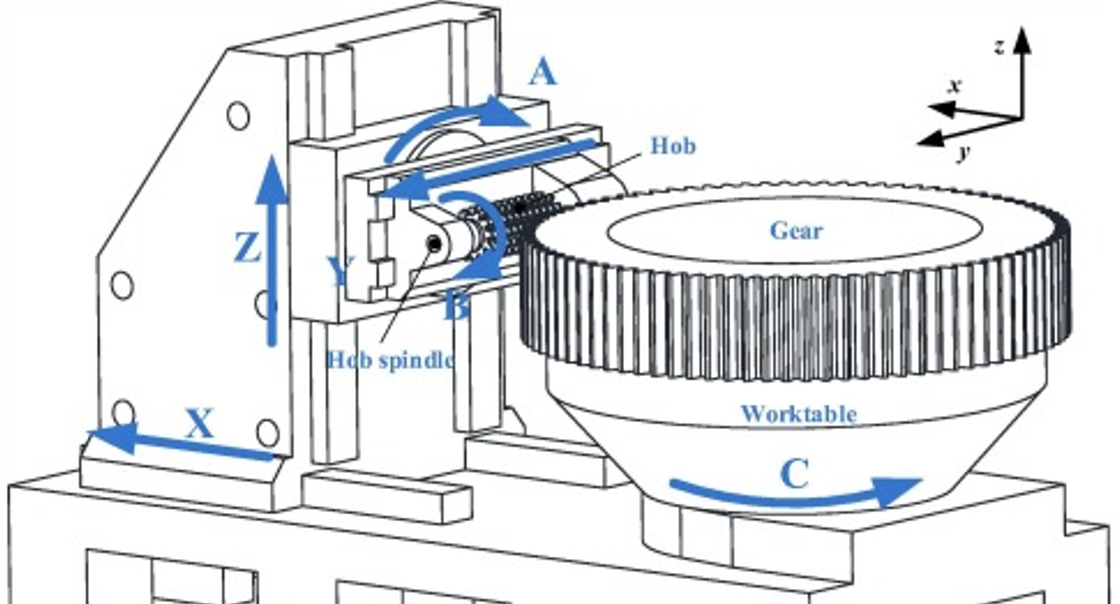
\includegraphics[width=12cm]{maschine_frei}
	\caption[Kinematik der Maschine]{Kinematik der Maschine mit Vorzeichenrichtung der Achsen; das Koordinatensystem ist Maschinenbett-fest}
	\label{fig:maschine}
\end{figure}

\subsection[Werkstück]{Kinematik der Werkstück-Seite}

Für die kinematische Kette auf der Werkstückseite gehen in die Gleichungen \ref{eq:werkstuckv1} und \ref{eq:werkstuckv2} ein Offset des Werkstückkoordinatensystems zum Maschinenkoordinatensystem $\mathbf{p}_{\mathrm{offset}} = \tranvec{a}{b}{c}$ und der Verdrehwinkel $C$ ein.
Der Offset erlaubt es ein versetztes Aufspannen des Werkstücks darzustellen und ist im idealen Fall ein Nullvektor.
Dem Verdrehwinkel wird ein weiterer Offest $\gamma$ aufgeprägt.
Dieser stellt den Fehler des verdrehten Aufspannens dar und erlaubt die Position von Zahn und Zahnlücke des virtuellen Schneckengetriebes zu korrigieren.
$C$ ist außerdem Funktion des Werkzeugwinkels und des Achsvorschubess.
Der Achsvorschub der $C$-Achse ist das Übersetzungsverhältnis des gedachten Schneckengetriebes.

\begin{equation*}
	\feed{C}{WSt} = \frac{n_{Schneidreihen}}{n_{Z"ahne}}
\end{equation*}

Die vollständige Formulierung des Werkstückwinkels $C$ lautet:

\begin{equation}
	\label{eq:wrkstwinkel}
	C = B \cdot{} \feed{C}{WSt} + \gamma
\end{equation}

Die Kinematik kann durch Änderung der Reihenfolge der Freiheitsgrade auf zwei verschiedene Arten aufgebaut werden.
Bei Variante 1 liegt das Bauteil zentriert auf dem Bearbeitungstisch, der sich um die C-Achse dreht.
Allerdings gehen die X-,Y- und Z-Achse nicht durch Mittelpunkt des Werkstücktisches sondern sind um $\mathbf{p}_{\mathrm{offset}}$ versetzt.
Bei Variante 2 liegt das Bauteil nicht zentrisch auf dem Bearbeitungstisch, der sich um die C-Achse dreht, sondern ist um $\mathbf{p}_{\mathrm{offset}}$ versetzt.
Die X-,Y- und Z-Achse starten dann im Mittelpunkt des Bearbeitungstisches.

\subsubsection[versetzter Bearbeitungstisch]{Variante 1: versetzter Bearbeitungstisch}

Die Transformation beschreibt die Position eines Werkstückpunktes im Koordinatensystems des Maschinenbettes.

\begin{equation}
	\label{eq:werkstuckv1}
	\vec{p}_\mathrm{m} = \transtm{a}{b}{c}
			\cdot{} \rottm{0}{0}{C}
			\cdot{} \vec{p}_\wst
\end{equation}

\subsubsection[versetztes Werkstück]{Variante 2: versetztes Werkstück}

\begin{equation}
	\label{eq:werkstuckv2}
	\vec{p}_\mathrm{m} =
					\rottm{0}{0}{C}
			\cdot{} \transtm{a}{b}{c}
			\cdot{} \vec{p}_\wst
\end{equation}


\subsection[Werkzeug]{Kinematik der Werkzeug-Seite}

Die kinematische Kette der Werkzeugseite \ref{eq:werkzeug} beinhaltet die verfahrbaren Achsen der Maschine mit ihrem jeweiligen Freiheitsgrad ein.
Dabei wird dem y-Achsenfreiheitsgrad ein Offset aufgeprägt, mit dem der Bereich des Werkzeuges im Eingriff verschoben werden kann.
Das Werkzeug unterliegt beim Schneiden Verschleiß.
Das Werkzeug ist länger als erforderlich und durch Verschieben des Werkzeugs entlang der y-Achse kann der Verschleiß gleichmäßig auf das Werkzeug verteilt werden.

\begin{equation*}
	Y = y + B \cdot \feed{Y}{Wz} + \yshift
\end{equation*}

Da der Spanabfall in Drehrichtung des Werkzeugs erfolgen soll ist diese mathematisch negativ einzutragen.
Das Werkzeug hat außerdem ein eigenes Koordinatensystem, bei welchem sich die z-Achse entlang der Drehrichtung des Werkzeuges erstreckt.
Es bietet sich an, die Ausrichtung des Koordinatensystems durch Drehung um $\pi/2$ um die x-Achse zu definieren.
So kann man mit sehr wenig Aufwand das Werkzeug in einem Polarkoordinatensystem anlegen und die Punktewolke in kartesische Koordinaten umrechnen.

\begin{equation}
	\label{eq:wkzgkoord}
	\vec{p}_{\mathrm{Wz,kart}} = \begin{pmatrix}  x = & r \cdot{} \cos{\phi}\\
											y = & r \cdot{} \sin{\phi}\\
											z = & h\end{pmatrix}
\end{equation}

\begin{figure}
	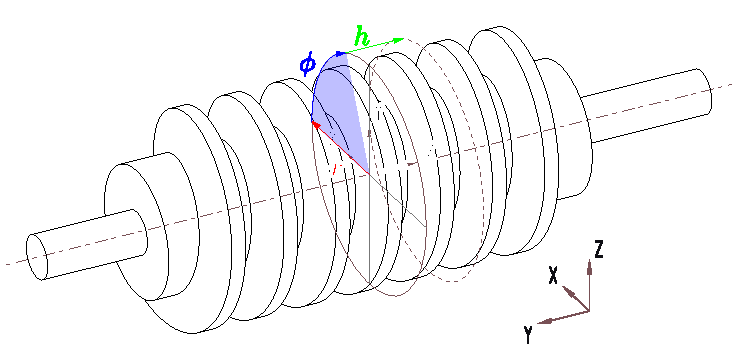
\includegraphics{hobspindle_coord}
	\caption{Ausrichtung des Werkzeugkoordinatensystems}
	\label{fig:hobspindle_coord}
\end{figure}

Die Transformation beschreibt die Position eines Werkzeugpunktes im Koordinatensystems des Maschinenbettes.

\begin{equation}
	\label{eq:werkzeug}
	\vec{p}_\mathrm{m} =  \transtm{X}{0}{Z}
			\cdot{} \rottm{A}{0}{0}
			\cdot{} \transtm{0}{Y}{0}
			\cdot{} \rottm{0}{-B}{0}
			\cdot{} \rottm{\pi/2}{0}{0}
			\cdot{} \vec{p}_\wz
\end{equation}

Zur Verdeutlichung, die ausformulierte Form der Transformationsmatrix zur Drehung des Werkzeugkoordinatensystems lautet:

\begin{equation*}
	\rottm{\pi/2}{0}{0}
	= \begin{bmatrix}1 & 0 & 0 & 0\\0 & 0 &-1 & 0\\0 & 1 & 0 & 0\\0 & 0 & 0 & 1\end{bmatrix}
\end{equation*}


Zur Vereinfachung der entstehenden Terme bietet sich das Zusammenfassen der Transformationsmatrizen zu einer Transformationsmatrix von Maschinenbett- in Werkzeugkoordinaten an:

\begin{equation*}
	T^\wz_\mathrm{m} = \transtm{X}{0}{Z}
				\cdot{} \rottm{A}{0}{0}
				\cdot{} \transtm{0}{Y}{0}
				\cdot{} \rottm{0}{-B}{0}
				\cdot{} \rottm{\pi/2}{0}{0}
\end{equation*}


\subsection[Vorschübe]{Aufprägung der Vorschübe auf die Achskoordinaten}

Durch die Natur der Fertigung von Verzahnung vergleichbar mit einem Schneckengetriebe hängen die Vorschübe der Achsen von der Rotation des Werkzeugs ab.
Dazu wird die Abhängigkeit der Achskoordinaten vom Werkzeugwinkel als Produkt des Werkzeugwinkels und einem Vorschubfaktor beschrieben.
Den x-Achsen und z-Achsen Koordinaten wird zusätzlich als linearer Offset die Position der x-Achse von einem Ausgangszustand aufgeprägt.
Bei der C-Achse ist dieser Effekt bereits mit dem Winkeloffset $\gamma$ realisiert.

\begin{itemize}
	\item{x-Axchse}
		\begin{equation}
			\label{eq:xaxisfun}
			X = x + B \cdot \feed{X}{Wz}
		\end{equation}

	\item{z-Axchse}
		\begin{equation}
			\label{eq:zaxisfeedrate}
			Z = z + B \cdot \feed{Z}{Wz}
		\end{equation}
\end{itemize}

Erläuterung der Nomenklatur für Vorschub-Variablen anhand Gl. \ref{eq:zaxisfeedrate}. Die Vorschübe beziehen sich immer auf die Drehung des Werkzeuges.
\begin{itemize}
	\item $f$: Vorschub (engl.: feed rate)
	\item $\mathrm{Z}$: Achsrichtung (Maschinen Z-Achse)
	\item $\wz$: bezogen auf die Werkzeugrotation
	\item $\mathrm{rad}$: Einheit (Bogenmaß)
\end{itemize}
Der Faktor lässt sich also definieren als Vorschub auf der z-Achse pro 1 Umdrehung des Werkzeugs $(2 \cdot \pi)$.

Damit ergibt sich für die Transformationsmatrix von Maschinenbett- nach Werkzeugkoordinaten in ausführlicher Form:

\begin{equation*}
	\mathbf{T}^\wz_\mathrm{m} = \transtm{x + B \cdot \feed{X}{Wz}}
								{0}
								{z + B \cdot \feed{Z}{Wz}}
				\cdot{} \rottm{A}{0}{0}
				\cdot{} \transtm{0}
								{y + B \cdot \feed{Y}{Wz} + \yshift}
								{0}
				\cdot{} \rottm{0}{-B}{0}
				\cdot{} \rottm{\pi/2}{0}{0}
\end{equation*}

\subsection[Gesamt]{Transformation von Werkzeug- in Werkstückkoordinaten}

Um die Transformation aus dem Werkzeug- in das Werkstückkoordinatensystem zu erhalten setzen wir die beiden Transformationsschritte gleich:

\begin{equation*}
			\transtm{a}{b}{c}
	\cdot{} \rottm{0}{0}{C}
	\cdot{} \mathbf{p}_\wst =
			\transtm{X}{0}{Z}
	\cdot{} \rottm{A}{0}{0}
	\cdot{} \transtm{0}{Y}{0}
	\cdot{} \rottm{0}{-B}{0}
	\cdot{} \rottm{\pi/2}{0}{0}
	\cdot{} \mathbf{p}_\wz
\end{equation*}

Die Gleichung wird durch Multiplikation mit den Inversen der Transformation- und Rotationsmatrix aufgelöst, sodass die Beschreibung der Transformation von Werkzeug- in Werkstückkoordinaten entsteht.

\begin{equation*}
	\begin{split}
				\rottm{0}{0}{-C}
		\cdot{} \transtm{-a}{-b}{-c}
		\cdot{} \transtm{X}{0}{Z}
		\cdot{} \rottm{A}{0}{0}
		\cdot{} \transtm{0}{Y}{0}
		\cdot{} \rottm{0}{-B}{0}
		\cdot{} \rottm{\pi/2}{0}{0}
		\cdot{} \mathbf{p}_\wz & =
				\mathbf{p}_\wst
		\\
				\mathbf{T}^\wz_\wst
		\cdot{} \mathbf{p}_\wz & =
	\end{split}
\end{equation*}

Die Transformationsmatrix wird ausmultipliziert:

\begin{align*}
	\mathbf{T}^\wz_\wst = &
	\rottm{0}{0}{-C}
	\cdot{} \transtm{-a}{-b}{-c}
	\cdot{} \transtm{X}{0}{Z}
	\cdot{} \rottm{A}{0}{0}
	\cdot{} \transtm{0}{Y}{0}
	\cdot{} \rottm{0}{-B}{0}
	\cdot{} \rottm{\pi/2}{0}{0}
	\\= &
	\rottm{0}{0}{-C}
	\cdot{} \transtm{X - a}{-b}{Z - c}
	\cdot{} \rottm{A}{0}{0}
	\cdot{} \transtm{0}{Y}{0}
	\cdot{} \rottm{0}{-B}{0}
	\cdot{} \rottm{\pi/2}{0}{0}
	\\= & \resizebox{.9 \hsize}{!}{$
		\rottm{0}{0}{-(B \cdot{} \feed{C}{WSt} + \gamma)}
		\cdot{} \transtm{x + B \cdot \feed{X}{Wz} -a}{-b}{z + B \cdot \feed{Z}{Wz} -c}
		\cdot{} \rottm{A}{0}{0}
		\cdot{} \transtm{0}{y + B \cdot \feed{Y}{Wz} + \yshift}{0}
		\cdot{} \rottm{0}{-B}{0}
		\cdot{} \rottm{\pi/2}{0}{0}$}
	\\= & \resizebox{.9 \hsize}{!}{$
		\begin{bmatrix}
			\sigma_2  \cdot \c{B}-\sigma_1  \cdot \s{A} \cdot \s{B} & -\sigma_2  \cdot \s{B}-\sigma_1  \cdot \c{B} \cdot \s{A} & -\sigma_1  \cdot \c{A} & \yshift  \cdot \sigma_1  \cdot \c{A} + x \cdot \sigma_2 -a +B \cdot \feed{X}{Wz}  \cdot \sigma_2 +y \cdot \sigma_1  \cdot \c{A}+B \cdot \feed{Y}{Wz}  \cdot \sigma_1  \cdot \c{A}\\
			-\sigma_1  \cdot \c{B}-\sigma_2  \cdot \s{A} \cdot \s{B} & \sigma_1  \cdot \s{B}-\sigma_2  \cdot \c{B} \cdot \s{A} & -\sigma_2  \cdot \c{A} & \yshift  \cdot \sigma_2  \cdot \c{A} - x \cdot \sigma_1 -b -B \cdot \feed{X}{Wz}  \cdot \sigma_1 +y \cdot \sigma_2  \cdot \c{A}+B \cdot \feed{Y}{Wz}  \cdot \sigma_2  \cdot \c{A}\\
			\c{A} \cdot \s{B} & \c{A} \cdot \c{B} & -\s{A} & \yshift \cdot \s{A} + z - c + B \cdot \feed{Z}{Wz} + y \cdot \s{A} + B \cdot \feed{Y}{Wz}  \cdot \s{A}\\
			0 & 0 & 0 & 1
		\end{bmatrix}$}\\
	\text{wobei:}\\
	& \quad \sigma_1 =\mathrm{sin}\left(\mathrm{ga}+B \cdot \feed{C}{WSt} \right)\\
	& \quad  \sigma_2 =\mathrm{cos}\left(\mathrm{ga}+B \cdot \feed{C}{WSt} \right)\\
	& \quad \s{\alpha} = \sin{(\alpha)}\\
	& \quad \c{\beta} = \cos{(\beta)}
\end{align*}

Zur Vereinfachung der mathematischen Notation wird der Transformationsmatrix $\mathbf{T}^\wz_\wst$ eine charakteristische Bezeichnung gegeben.
$\mathbf{G}$ steht hierbei für \textit{Gesamt}.

\begin{equation*}
	\mathbf{T}^\wz_\wst = \mathbf{G}
\end{equation*}

Es folgt für die Beschreibung eines Punktes mit Werkzeugkoordinaten in Maschinenkoordinaten:

\begin{equation*}
	\mathbf{p}_\wst = \mathbf{G} \cdot{} \mathbf{p}_\wz
\end{equation*}

\section[Lösung]{Lösung der relevanten Gleichung}

Bei dem gewählten Lösungsverfahren des Problems soll der Werkzeugwinkel in Abhängigkeit von einer vorgegebenen Höhe eines Werkzeugpunktes in z-Richtung bestimmt werden.
Es gilt die Formel zu lösen die sich bei Anwendung der allgemeinen Transformationsmatrix auf einen Werkzeugpunkt in der z-Komponente des Ergebnisses ergibt.

\subsection[Polarkoordinaten]{Werkzeug in Polarkoordinaten definiert}

\begin{equation*}
			\begin{pmatrix} p_{\wst,x} \\ p_{\wst,y} \\ p_{\wst,z} \\ 1 \end{pmatrix}
	= \mathbf{G}
		\cdot{} \begin{pmatrix} r_\wz \cdot{} \cos{\phi} \\ r_\wz \cdot{} \sin{\phi} \\ h_\wz \\ 1 \end{pmatrix}
\end{equation*}

Die Lösung der Gleichung soll für einen vorgebenen Wert in z-Richung erfolgen.
\begin{equation*}
	\begin{split}
		p_{\wst,z} = z_{soll} = Z - c + B \cdot{} \feed{Z}{Wz} + & \sin(A) \cdot{} (Y + \yshift + B \cdot{} \feed{Y}\wz) \\
							- & \sin(A) \cdot{} h_\wz \\
							+ & \cos(A) \cdot{} r_\wz \cdot{} \sin(\phi_\wz) \cdot{} \cos(B)\\
							+ & \cos(A) \cdot{} r_\wz \cdot{} \cos(\phi_\wz) \cdot{} \sin(B)
	\end{split}
\end{equation*}

Da die Lösung der Gleichung durch Finden des Nullpunktes erfolgen soll, muss die Gleichung nach dem Werkzeugwinkel $B$ aufgelöst werden.
\begin{equation*}
	\begin{split}
		0 = Z - c -z_{soll} + B \cdot{} \feed{Z}{Wz} + & \sin(A) \cdot{} (Y + \yshift + B \cdot{} \feed{Y}{Wz} - h_\wz) \\
			+ & \cos(A) \cdot{} r_\wz \cdot{} \sin(\phi_\wz) \cdot{} \cos(B) \\
			+ & \cos(A) \cdot{} r_\wz \cdot{} \cos(\phi_\wz) \cdot{} \sin(B)
	\end{split}
\end{equation*}

\begin{equation}
	\label{eq:additionsterm}
	\sin(x_1 \pm x_2) = \sin(x_1) \cdot{} \cos(x_2) \pm \cos(x_1) \cdot{} \sin(x_2)
\end{equation}

Gemäß dem Additionsterm \ref{eq:additionsterm} aus \cite[Gleich. 7.6.1]{Papula2017} können die $\sin$- und $\cos$-Terme in den beiden Summanden mit $cos(A) \cdot r_\wz$ zusammengefasst werden.

\begin{align*}
	0 = Z - c  - z_{soll} + B \cdot{} \feed{Z}{Wz} + & \sin(A) \cdot{} (Y + \yshift + B \cdot{} \feed{Y}{Wz} - h_\wz) \\
												   + & \cos(A) \cdot{} r_\wz \cdot{} \sin(B + \phi_\wz) \\
	\intertext{Von beiden Seite wird $r_\wz \cdot{} \cos(A) \cdot{} \sin(B + \phi_\wz)$ subtrahiert:}
	-r_\wz \cdot{} \cos(A) \cdot{} \sin(B + \phi_\wz) = & \\
			Z - c  - z_{soll} + B \cdot{} \feed{Z}{Wz} + & \sin(A) \cdot{} (Y + \yshift + B \cdot{} \feed{Y}{Wz} - h_\wz)\\
\end{align*}

Nun wird durch $r_\wz \cdot{} \cos(A)$ geteilt:

\begin{equation*}
	\sin(B + \phi_\wz) = -\frac{Z - c  - z_{soll} + B \cdot{} \feed{Z}{Wz} + \sin(A) \cdot{} (Y + \yshift + B \cdot{} \feed{Y}{Wz} - h_\wz)}
	{r_\wz \cdot{} \cos(A)}
\end{equation*}

\begin{equation}
	B + \phi_\wz = \arcsin{\left(-\frac{Z - c  - z_{soll} + B \cdot{} \feed{Z}{Wz} + \sin(A) \cdot{} (Y + \yshift + B \cdot{} \feed{Y}{Wz} - h_\wz)}
		{r_\wz \cdot{} \cos(A)}\right)}
\end{equation}

\begin{equation}
	\label{eq:arcsinpunktsymm}
	\arcsin{-x} = -\arcsin{x}
\end{equation}

Wegen der Punktsymmetrie des Arkussinus \ref{eq:arcsinpunktsymm} ergibt sich:
\begin{equation}
	B = -\phi_\wz -\arcsin{\left(\frac{Z - c  - z_{soll} + B \cdot{} \feed{Z}{Wz} + \sin(A) \cdot{} (Y + \yshift + B \cdot{} \feed{Y}{Wz} - h_\wz)}
		{r_\wz \cdot{} \cos(A)}\right)}
\end{equation}


Lösung:
\begin{equation}
	B = \pi - \phi_\wz + \arcsin{\left(\dfrac{Z - c - z_{soll} + B_0 \cdot{} \feed{Z}{Wz} + \sin(A) \cdot{} (Y + \yshift + B_0 \cdot{} \feed{Y}{Wz} - h_\wz)}
		{r_\wz \cdot{} \cos(A)}\right)}
\end{equation}

\subsection[kartesische Koordinaten]{Werkstück in kartesischen Koordinaten definiert}

\begin{equation}
	\begin{pmatrix}p_{\wst,x}\\p_{\wst,y}\\p_{\wst,z}\\1\end{pmatrix} = \mathbf{G} \cdot{} \begin{pmatrix}p_{\wz,x}\\p_{\wz,y}\\p_{\wz,z}\\1\end{pmatrix}
\end{equation}

\begin{equation*}
	\begin{split}
		p_{\wst,z} = z_{soll} = z - c + B \cdot{} \feed{Z}{Wz} + & \sin(A) \cdot{} (y + \yshift + B \cdot{} \feed{Y}{Wz}) \\
							- & \sin(A) \cdot{} z_\wz \\
							+ & \cos(A) \cdot{} y_\wz \cdot{} \cos(B) \\
							+ & \cos(A) \cdot{} x_\wz \cdot{} \sin(B) | -z_{soll}
	\end{split}
\end{equation*}


\begin{equation}
	\begin{split}
		0 = z - c - z_{soll} + B \cdot{} \feed{Z}{Wz} + & \sin(A) \cdot{} (y + \yshift + B \cdot{} \feed{Y}{Wz} - z_\wz) \\
												+ & \cos{(A)} \cdot{} (y_\wz \cdot{} \cos(B) + x_\wz \cdot{} \sin(B))
	\end{split}
\end{equation}

Mit:
\begin{equation}
	\begin{split}
		\beta & = z - c - z_{soll} + B \cdot{} \feed{Z}{Wz}\\
		\alpha &= y + \yshift + B \cdot{} \feed{Y}{Wz} - z_\wz
	\end{split}
\end{equation}

\begin{equation}
	\begin{split}
		0 = \beta +
			\sin(A) \cdot{} \alpha +
			\cos{(A)} \cdot{} (y_\wz \cdot{} \cos(B) + x_\wz \cdot{} \sin(B)) | - \cos{(A)} \cdot (\dots)
	\end{split}
\end{equation}

\begin{equation}
	(-1) \cdot (\cos{(A)} \cdot{} (y_\wz \cdot{} \cos(B) + x_\wz \cdot{} \sin(B))) = 
	\beta +	\sin(A) \cdot{} \alpha | \cdot (-1) \cdot \frac{1}{\cos{A}}
\end{equation}

\begin{equation}
	y_\wz \cdot{} \cos(B) + x_\wz \cdot{} \sin(B) = 
	(-1) \cdot \left(
	\frac{\beta}{\cos{(A)}} +
	\frac{\sin(A)}{\cos{(A)}} \cdot{} \alpha \right) \quad | \cdot \frac{1}{\cos{(B)}}
\end{equation}

\begin{equation}
	y_\wz + x_\wz \cdot{} \frac{\sin(B)}{\cos{B}} = 
	(-1) \cdot \left(
	\frac{\beta}{\cos{A} \cdot \cos{B}} +
	\frac{\sin(A)}{\cos{A} \cdot \cos{B}} \cdot{} \alpha \right)
\end{equation}

\begin{equation}
	(-1) \cdot (y_\wz + x_\wz \cdot{} \frac{\sin(B)}{\cos{(B)}}) = 
	\frac{\beta}{\cos{(A)} \cdot \cos{(B)}} +
	\frac{\tan{(A)}}{\cos{(B)}} \cdot{} (y + \yshift + B \cdot{} \feed{Y}{Wz} - z_\wz) | + y_\wz
\end{equation}

\begin{equation}
	- x_\wz \cdot{} \tan{B} = 
	\frac{\beta}{\cos{(A)} \cdot \cos{(B)}} +
	\frac{\tan{(A)}}{\cos{(B)}} \cdot{} (y + \yshift + B \cdot{} \feed{Y}{Wz} - z_\wz) + y_\wz
\end{equation}

\begin{equation}
	\tan{x} = \frac{\sin{x}}{\cos{x}}
\end{equation}

\begin{equation}
	\begin{split}
		0 = z - c - z_{soll} + B \cdot{} \feed{Z}{Wz} + & \sin(A) \cdot{} (y + \yshift + B \cdot{} \feed{Y}{Wz} - z_\wz) \\
		+ & \cos{(A)} \cdot{} (y_\wz + x_\wz \cdot{} \tan(B))
	\end{split}
\end{equation}

\begin{equation}
	\begin{split}
		-\cos{(A)} \cdot{} (y_\wz + x_\wz \cdot{} \tan(B)) = & \\
		 z - c - z_{soll} + B \cdot{} \feed{Z}{Wz} + & \sin(A) \cdot{} (y + \yshift + B \cdot{} \feed{Y}{Wz} - z_\wz) \\
	\end{split}
\end{equation}

\begin{equation}
	y_\wz + x_\wz \cdot{} \tan(B) = -\frac{z - c - z_{soll} + B \cdot{} \feed{Z}{Wz} + \sin(A) \cdot{} (y + \yshift + B \cdot{} \feed{Y}{Wz} - z_\wz)}{\cos{(A)}}
\end{equation}

\begin{equation}
	x_\wz \cdot{} \tan(B) =
					-\frac{z - c - z_{soll} + B \cdot{} \feed{Z}{Wz}}{\cos{(A)}}
					- y_\wz
					- \frac{\sin(A)}{\cos{(A)}} \cdot{} (y + \yshift + B \cdot{} \feed{Y}{Wz} - z_\wz)
\end{equation}

\begin{equation}
	\tan(B) = -\frac{z - c - z_{soll} + B \cdot{} \feed{Z}{Wz}}{\cos{(A)} \cdot{} x_\wz}
				- \frac{y_\wz}{x_\wz}
				- \tan{(A)} \cdot{} \frac{y + \yshift + B \cdot{} \feed{Y}{Wz} - z_\wz}{x_\wz}
				| \arctan{()}
\end{equation}

\begin{equation}
	B = -\arctan{\left(\frac{z - c - z_{soll} + B \cdot{} \feed{Z}{Wz}}{\cos{(A)} \cdot{} x_\wz} +\frac{y_\wz}{x_\wz}\right)}
		- A \cdot{} \frac{y + \yshift + B \cdot{} \feed{Y}{Wz} - z_\wz}{x_\wz}
\end{equation}
